%% ELEC 451 - Lab 1 report
%% IEEEtran, single column (full page width, no columns).
%% Fill in your student numbers where marked TODO and replace the
%% placeholder sections with your content. Figures go in Images/.

\documentclass[journal,onecolumn]{IEEEtran}

% *** MATH ***
\usepackage{amsmath}

% *** FIGURES ***
\usepackage{graphicx}
\usepackage{float}
\graphicspath{{Images/}{./}}

% *** PDF, URL AND HYPERLINK PACKAGES ***
\usepackage{hyperref}

% correct bad hyphenation here
\hyphenation{op-tical net-works semi-conduc-tor}

% *** SECTION HEADINGS *** bigger main section titles (keep IEEE centered small-caps)
\makeatletter
\renewcommand\section{\@startsection{section}{1}{\z@}%
  {3.0ex plus 1.5ex minus 1.5ex}%
  {0.7ex plus 1ex minus 0ex}%
  {\normalfont\Large\centering\scshape}}
\makeatother

\begin{document}

% paper title
\title{ELEC 451 Power Electronics\\
Lab 1: Power Quality and Basic Uncontrolled Rectifiers}

% TODO: fill in student numbers
\author{Christian Conroy, \_\_\_\_\_\_\_\_\_, % TODO: student number
        Labib Kowsar, \_\_\_\_\_\_\_\_\_, % TODO: student number
        Didier Gil Martinez, \_\_\_\_\_\_\_\_\_ % TODO: student number
}

% The report headers
\markboth{ELEC 451 Power Electronics. Lab Report 1, October 2026}%
{ELEC 451 Power Electronics. Lab Report 1, October 2026}

% make the title area
\maketitle

\begin{center}
\today
\end{center}

%% ====================================================================
\section{Introduction}
\label{sec:intro}

% TODO: write introduction (objectives, the three rectifier circuits, report organization).

%% ====================================================================
\section{Simulation}
\label{sec:sim}

% Vs = 12 Vrms, Fs = 60 Hz; Ls = 1 mH, Rs = 2 Ohms, L = 1 mH, C = 50 uF, R = 500 Ohms, Rshunt = 1 Ohm.
% For each circuit: plot vs, vd, is, iL; crest factor, THD, DPF/PF.

\subsection{Circuit 1 --- Full-Bridge Rectifier with Resistive Load}
\label{sec:sim-c1}

% TODO: schematic, waveforms (vs, vd, is, iL), crest factor, THD, DPF/PF, comments.

%\begin{figure}[H]
%\centering
%\includegraphics[width=\textwidth]{circuit1_waveforms.png}
%\caption{Short one-sentence caption.}
%\label{fig:sim-c1}
%\end{figure}

\subsection{Circuit 2 --- Full-Bridge Rectifier with Capacitive Filter and Resistive Load}
\label{sec:sim-c2}

% TODO: schematic, waveforms (vs, vd, is, iL), crest factor, THD, DPF/PF, comments.

\subsection{Circuit 3 --- Full-Bridge Rectifier with LC Filter and Resistive Load}
\label{sec:sim-c3}

\begin{figure}[H]
\centering
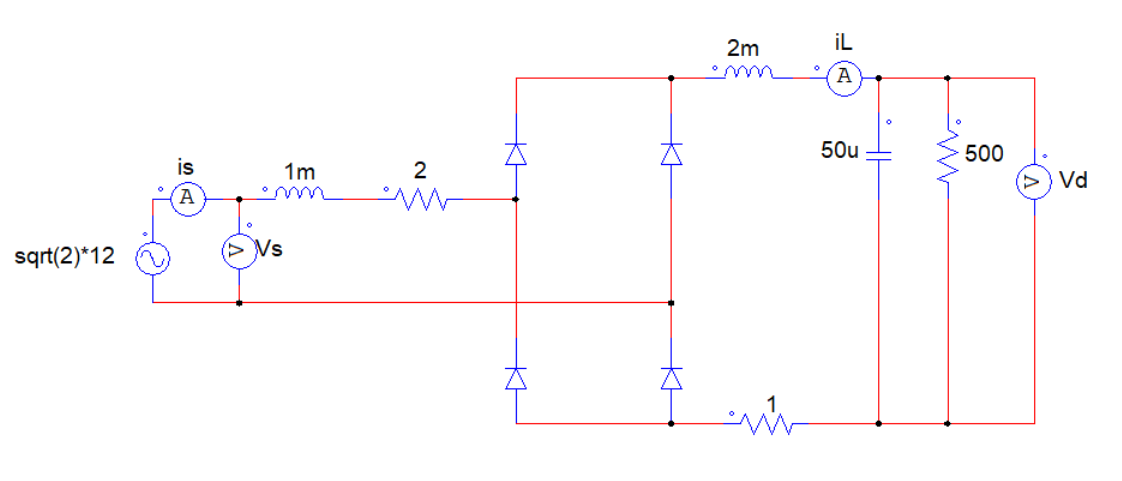
\includegraphics[width=0.85\textwidth]{sim_circuit3_schematic.png}
\caption{PSIM schematic of Circuit 3.}
\label{fig:sim-c3-schem}
\end{figure}

The THD can be calculated as (these are the source voltage and current):
\begin{equation}
\mathrm{THD} = \frac{\sqrt{\sum_{h \ne 1} I_{sh}^2}}{I_{s1}}
\end{equation}

equivalently...
\begin{equation}
I_s = I_{s1}\sqrt{1 + \mathrm{THD}^2}
\end{equation}
\begin{equation}
\frac{I_s^2}{I_{s1}^2} - 1 = \mathrm{THD}^2
\end{equation}

where $I_{s1}$ is the fundamental frequency of the source current.

We know at steady state, the $I_s = I_L = I_o$.
And since the load determines how much current flows through from the source,
\begin{equation}
I_{s1} = \frac{V_s}{R + R_{\mathrm{shunt}}}
\end{equation}
\begin{equation}
I_{s1} = \frac{12~\mathrm{V}}{500 + 1}
\end{equation}
\begin{equation}
\boxed{I_{s1} = 23.95~\mathrm{mA}}
\end{equation}
This is the fundamental component of $I_{s,\mathrm{RMS}}$ since the harmonic distortion comes from the current ripple.

%% ====================================================================
\section{Experiment}
\label{sec:exp}

% Same three circuits on the uncontrolled rectifier board; vs = 12 Vrms.
% vs via differential probe, is via current probe, vd and iL (at shunt) via regular probes.

\subsection{Circuit 1 --- Resistive Load}
\label{sec:exp-c1}

% TODO: time-domain and FFT captures, measurements, calculations, comments.

\subsection{Circuit 2 --- Capacitive Filter and Resistive Load}
\label{sec:exp-c2}

% TODO: time-domain and FFT captures, measurements, calculations, comments.

\subsection{Circuit 3 --- LC Filter and Resistive Load}
\label{sec:exp-c3}

% TODO: time-domain and FFT captures, measurements, calculations, comments.

%% ====================================================================
\section{Conclusion}
\label{sec:conc}

% TODO: summary of findings (simulation vs experiment).

\end{document}
